Date : 14 december 2023

\subsubsection{Amplitude Shift Keying 'ASK'}

Voordelen:
\begin{itemize}
  \item Eenvoudig en goedkoop.
  \item Weinig bandbreedte nodig.
\end{itemize}

Nadelen:
\begin{itemize}
  \item Referentieniveau is lastig vast te stellen.
  \item Gevoelig voor amplitudeverstoring (overeenkomstig met AM).
\end{itemize}

\begin{figure}[H]
\centering
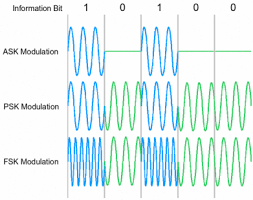
\includegraphics[scale=0.8]{vormen van modulatie.png}
\caption{Vormen van modulatie}
\end{figure}

\subsubsection{Phase Shift Keying 'PSK,QPSK'}

Er zijn verschillende methodes van PSK zoals:
\begin{itemize}
  \item Binaire Phase Shift Keying (`BPSK') $\Rightarrow$ 1-bit symbool
  \item Quadrature Phase Shift Keying (`QPSK') $\Rightarrow$ 2-bit symbool
  \item Enzv.
\end{itemize}

BPSK is de eenvoudigste vorm van PSK met '1 bit per symbool'. Het constellatiediagram (IQ) van BPSK ziet er als volgt uit:
\begin{itemize}
  \item Een '1' $\Rightarrow$ 0°
  \item Een '0' $\Rightarrow$ 180°
\end{itemize}

\begin{figure}[H]
\centering
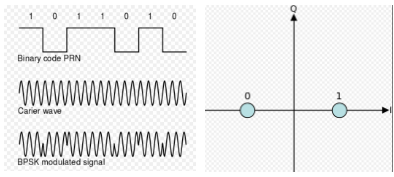
\includegraphics[scale=0.8]{BPSK.png}
\caption{BPSK}
\end{figure}

\begin{figure}[H]
\centering
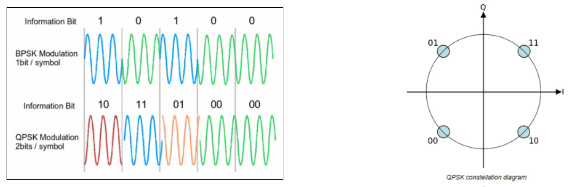
\includegraphics[scale=0.8]{QPSK.png}
\caption{Quadrature Phase Shift Keying}
\end{figure}

\subsubsection{Klokextractie}

Klokextractie vs. Demodulatie
\begin{itemize}
  \item Om de verzonden data uit het gemoduleerde signaal te kunnen halen, is het noodzakelijk om de klokfrequentie waarmee verzonden is te kennen, de 'sample frequentie'.
  \item Dit proces noemen we klokextractie, waarbij de ontvanger wordt gesynchroniseerd met de zender.
  \item Wanneer er voldoende veranderingen in het gemoduleerde signaal aanwezig zijn, is het mogelijk de zendklok te extraheren uit het gemoduleerde signaal. De veranderingen in het gemoduleerde signaal corresponderen namelijk met de zendklok frequentie.
\end{itemize}

Klokextractie vs. Preamble
\begin{itemize}
  \item In de preamble kan vaak ook de klokfrequentie worden verkregen.
  \item Wat is dan een Preamble?
\end{itemize}

Voor een goede demodulatie is het dus noodzakelijk dat de ontvangstklok dezelfde frequentie krijgt als de zendklok. Nog belangrijker is dat de fase van de ontvangstklok in orde is!


\subsubsection{Quedrature Amplitude Modulation 'QAM'}
PSK is praktisch te gebruiken met maximaal 8 fases. Om meerdere levels te kunnen gebruiken wordt QAM toegepast.
Hierbij wordt een combinatie van amplitude en fasesprongen
gemaakt.

\begin{figure}[H]
\centering
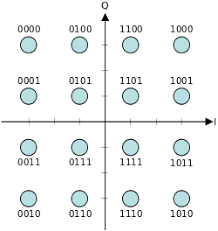
\includegraphics[scale=0.8]{Constelatiediagram.png}
\caption{Constellatie}
\end{figure}

\begin{figure}[H]
\centering
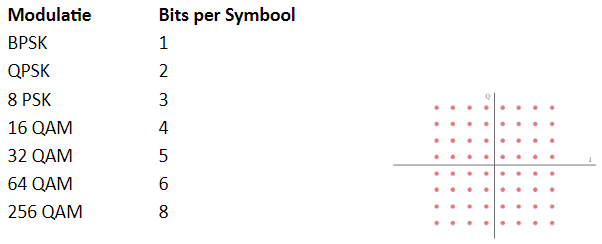
\includegraphics[scale=0.8]{Digitale modulatie overzicht.png}
\caption{Digitale modulatie: overzicht}
\end{figure}


\subsubsection{Transmissiepad en Parameters}

\begin{itemize}
    \item Zendvermogen: Het uitgangsvermogen van de zendunit, meestal
    uitgedrukt in dBm.
    \item RSSI ‘Received Signal Strength Indicator’: Het gemeten
    ontvangstniveau in de ontvangstunit. Meestal uitgedrukt in dBm.
    Met meer symbolen krijg je ook een hogere RSSI
    \item Receive Level: Meestal wordt hier een range mee aangeduid
    waarbinnen het ontvangstniveau moet liggen.
    \item S/R: ratio geeft de Signal to Noise Ratio aan. Meestal wordt van de
    ontvanger opgegeven welke S/R nodig is om een bepaalde BER te
    garanderen. De S/R wordt uitgedrukt in dB.
    \item Bandwidth: De bandbreedte van het RF signaal dat uit de zender
    komt.
    \item  BER: Bit Error Rate is de verhouding tussen het aantal foute
    ontvangen bits ten opzichte van het totaal aantal ontvangen bits.
    BER = (aantal foutieve bits) / (totaal aantal ontvangen bits)
    \item Interference: Verstoring van het ontvangstsignaal door andere
    zenders of door multipathfading.
    \item Attenuation (verzwakking): Demping die optreedt door bijvoorbeeld
    kabels, connectoren en de free space los.
    \item Phasedistortion: Fasevervorming die ontstaat door een verschil in
    looptijd(snelheid) van de aanwezige frequentiecomponenten in een
    pulsvorming signaal (dispersie).
  \end{itemize}


\subsubsection{LoRa}

\begin{figure}[H]
\centering
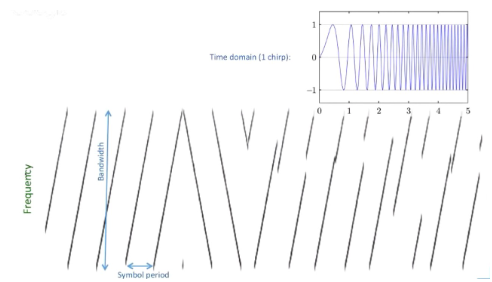
\includegraphics[scale=0.8]{LoRa chirp.png}
\caption{LoRa}
\end{figure}

\begin{figure}[H]
\centering
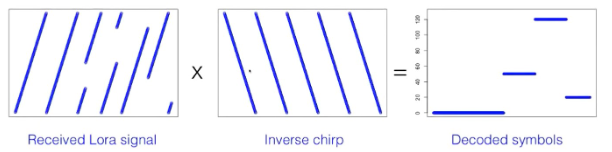
\includegraphics[scale=0.8]{LoRa Demodulatie.png}
\caption{LoRa}
\end{figure}
